\chapter{Week12}

\section{Monday}\index{Monday_lecture}
\subsection{Qualitative Theory}
Stability or ``equilibria'':
\[\dot{\X}=f(t,\X)
\]
If a solution $\X(t)$ is independent of $t$, i.e. $\dot{\X}\equiv0$ , then we call it equilibrium station. Thus, $\dot{\X}=f(t,\X)=0$ or $f(t,\xi)$ since $\X(t)=\xi$ for some constant $\xi$.\\
Autonomous system. $\dot{\X}=f(\X)\qquad f$ is independent of $t$.
\begin{example}
\begin{figure}[H]
\centering
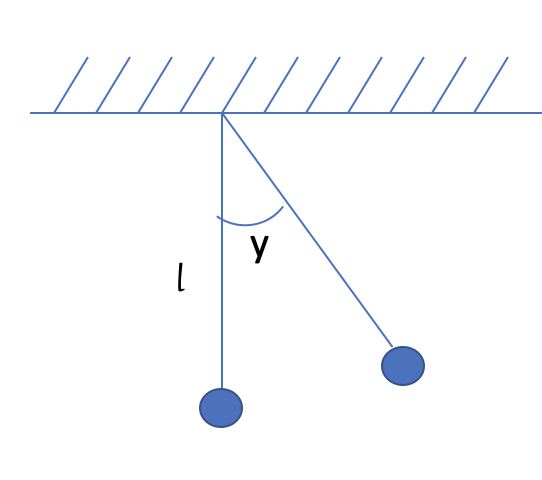
\includegraphics[width=5cm]{week12}
\end{figure}
tangential component:
\[F=-mg-siny=ma
\]
i.e
\[m(ly)\pp=-mg\sin y
\]
or
\[y\pp+\frac{g}{l}\sin y=0
\]
Let $\X=\begin{pmatrix}x_1\\x_2\end{pmatrix}$, where $x_1=y$, $x_2=y\p$
\[\X\p=\begin{pmatrix}x_1\p\\x_2\p\end{pmatrix}=\begin{pmatrix}y\p\\y\pp\end{pmatrix}=\begin{pmatrix}y\p\\-\frac{g}{l}\sin y\end{pmatrix}=\begin{pmatrix}x_2\\-\frac{g}{l}\sin x_1\end{pmatrix}
\]
Equilibira point: $\X\p=0$, i.e. \[\begin{pmatrix}x_2\\-\frac{g}{l}\sin x_1\end{pmatrix}\quad\Rightarrow\quad \X=\begin{pmatrix}k\pi\\0\end{pmatrix}\quad k\in\mathbb{Z}
\]
\end{example}
The equilibium solution $\xi$ is stable means:\\
``If $\X(0)$ is close to the equilibrium solution $\X(t)=\xi$, then $\X(t)$ stays close to the equilibrium solution $\xi$ for all $t>0$''\\
``For any given $\varepsilon>0, \exists~\delta>0$ s.t. for any $||\X(0)-\xi||<\delta$, we have $||\X(t)-\xi||<\varepsilon\quad\forall t>0$''
\begin{example}
In the last example (0,0) is stable since for every $\varepsilon>0$, $||\X(t)-(0,0)||<\varepsilon$ for all t, if $||\X(0)-(0,0)||<\delta$\\
$(\pi,0)$ is unstable because there exists $\varepsilon_0>0$ s.t. $\forall\delta>0$, we have $||x(t)-(x,0)||>\varepsilon_0$ for some $t>0$, with $||\X(0)-(x,0)||<\delta$. To show, pick $\varepsilon=\frac{\pi}{2}$, then $\forall\delta>0$, $||x(t_0)-(\pi,0)||=\pi>\frac{\pi}{2}=\varepsilon$

\end{example}
Let $\tilde{\X}(t)$ be a solution, then we say $\tilde{\X}(t)$ is stable if $\forall\varepsilon>0, \exists\delta>0$, s.t. a solution $\X(t)$ with $|\X(0)-\tilde{\X}(0)|<\delta$ satisfies $|\X(t)-\tilde{\X}(t)|<\varepsilon$ for all $t>0$.
\begin{figure}[H]
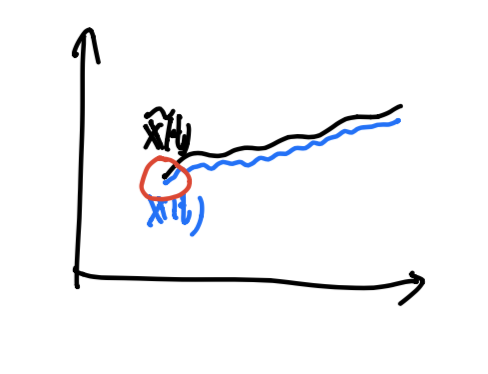
\includegraphics[width=5cm]{week12_2}
\end{figure}
Continuous dependence on initial value:\\
For any $T>0$ given and for any $\varepsilon>0$, there exists a $\eta>0$ s.t. $||\X(t)-\X^*(t)||<\varepsilon$ if $||\X(0)-\X^*(0)||<\eta$ for all $t<T$
\begin{figure}[H]
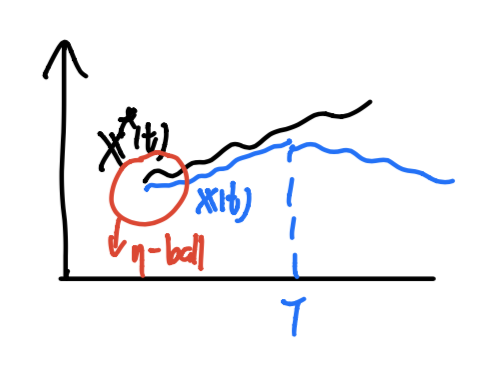
\includegraphics[width=5cm]{week12_3}
\end{figure}



Stability of linear system:\\
Consider   $ \dot{X}=AX$  where A is a matrix with constant coeffcient. \\

(i) If A has an eigenvalue with positive real root, then all solutions are countable. \\

(ii) If all eigenvalue of A have negative real part, then all soluions are stable. \\

(iii)Suppose $\lambda_1=i\delta_1, \lambda_2=i\delta_2, .... , \lambda_k=i\delta_n$ and $\lambda_{k+1}, .... ,\lambda_n$ are eigenvalues with negative real parts. Let $\lambda_j=i\delta_j, j=1, .... ,$ all solutions are mustable. \\
\begin{proof}
 (i) Assume A has an eigenvalue $\lambda=\alpha+i\beta,\ where\ \alpha>0.$ \\
Case 1: $\beta=0.$ Let v be the corresponding eigenvalue of $\lambda$. $X=e^{\alpha{t}}$ is a solution. $||X(t)||=||e^{\lambda{t}}v||=e^{\alpha{t}} \Rightarrow as\ t \to \infty.$\\
Then $||\delta X(t)||=\delta e^{\alpha{t}}||v|| \to \infty\ as\ t \to \infty$, Thus $||\delta X(0)-0||=||\delta X(0)||=\delta||v||,$ which implies solution is not stable.
\end{proof}








